\documentclass{article}

\usepackage{bookman}

% acentuação
\usepackage[utf8]{inputenc}
\usepackage{indentfirst}
\usepackage{xspace}
%\usepackage{chicago}
\usepackage{url}
\usepackage{setspace}
\usepackage{graphicx}
\usepackage[table,xcdraw]{xcolor}

\usepackage{fancybox}
\usepackage{amsmath}
\usepackage{amsfonts}
\usepackage[bbgreekl]{mathbbol}
\usepackage{amssymb}
\usepackage{url}
\usepackage{multirow}
\usepackage{booktabs}
\usepackage{paralist}

\usepackage{color}
\usepackage{subfigure}
\definecolor{red}{rgb}{0.9,0.1,0.1}
\definecolor{blue}{rgb}{0,0.1,0.8}

%%% cria links no arquivo .pdf
%%% comentar as linhas na versão para impressao
\usepackage[pdftex, plainpages=false, hyperfootnotes=false]{hyperref}
\hypersetup{colorlinks=true, linkcolor=blue, citecolor=blue, urlcolor=blue}

%%% bibliografia
%\usepackage{natbib}
\usepackage[sf,outermarks,clearempty]{titlesec}

\usepackage[pdftex]{geometry}
  \geometry{a4paper,left=3cm,right=2cm,top=3cm,bottom=3cm,twoside}

\usepackage{acronym}


\usepackage{eqparbox,array}

\usepackage{comment}
\usepackage{fontenc}
\usepackage{inputenc}
\usepackage{listing}
\usepackage{listings}
\usepackage{framed}
\usepackage{imakeidx}


\acrodef{CBIR}{Content-based image retrieval}
\acrodef{MAM}{Metric Access Method}
\acrodef{AM}{Access Method}
\acrodef{SAM}{Spatial Access Method}
\acrodef{MST} {Minimum Spanning Tree}
\acrodef{IR} {Information Retrieval}
\acrodef{NDC} {Number of Distance Calculations}
\acrodef{LAESA} {Linear Approximating Eliminating Search Algorithm}
\acrodef{AESA} {Approximating Eliminating Search Algorithm}
\acrodef{RNG} {Relative Neighborhood Graph}
\acrodef{DT} {Delaunay Triangulation}
\acrodef{GG} {Gabriel Graph}
\acrodef{UG} {Urquhart Graph}
\acrodef{SAT} {Spacial Approximation Tree}
\acrodef{RNDF} {Relative Neighborhood Density Factor}
\acrodef{NN} {Nearest Neighbor}
\acrodef{NAG} {Neighborhood Approximation Graph}
\acrodef{HRG} {Hyperspherical Region Graph}
\acrodef{NA-Graph} {Neighborhood Approximation Graph}
\acrodef{DA} {Disk Access}
\acrodef{DTW} {Dynamic Time Warping}
\acrodef{LSH} {Locality Sensitive Hashing}
\acrodef{CNN} {Convolutional Neural Network}
\acrodef{CNNs} {Convolutional Neural Networks}

%\newcommand{ \Correction }[ 1 ] {\textcolor{black}{#1}}
%\newcommand{ \NewMaterial }[ 1 ] {\textcolor{black}{#1}}
%\newcommand{ \ConnectDots }[ 1 ] {\textcolor{black}{#1}}
%\newcommand{ \NewMaterialGPU }[ 1 ] {\textcolor{black}{#1}}
%\newcommand{ \Error }[ 1 ] {\textcolor{black}{#1}}


\acrodef{CBIR} {Content-based Image Retrieval}
\acrodef{MAM}  {Métodos de Acceso Métrico}
\acrodef{SAM}  {Métodos de Acceso Espacial}
\acrodef{MAE}  {Métodos de Acesso Espaciais}

\acrodef{DTW}  {Dynamic Time Warping}
\acrodef{LSH}  {Locality Sensitive Hashing}
\newenvironment{Figure}
  {\par\medskip\noindent\minipage{\linewidth}}
  {\endminipage\par\medskip}

\usepackage{courier}
\definecolor{darkgreen}{rgb}{0,0.6,0.1}
\definecolor{gray}{rgb}{0.75,0.75,0.75}


\title{Approximate nearest neighbors by  deep  hashing on large-scale search: Comparison of representations and retrieval performance}

\author {}

\date{\today}
% Hint: \title{what ever}, \author{who care} and \date{when ever} could stand
% before or after the \begin{document} command
% BUT the \maketitle command MUST come AFTER the \begin{document} command!
 

\begin{document}

\tableofcontents
\maketitle

\begin{abstract} % aocsa
The growing volume of data and its increasing complexity require even more efficient and faster data mining techniques.  Numerous representation methods for dimensionality reduction and similarity measures geared towards  data mining have been introduced. 

An optimal data representation  is  an important  task in information retrieval.   A fast indexing method increases the performance level and a good representation offers precise discrimination.


The growing volume of data and its increasing complexity require even more efficient and faster data mining techniques.  Numerous representation methods for dimensionality reduction and similarity measures geared towards  data mining have been introduced.

An optimal data representation  is  an important  task in information retrieval.   A fast indexing method increases the performance level and a good representation offers precise discrimination.

Hashing produces  compact representation for  data, to perform task like classification or retrieval based on these short codes.

When hashing is supervised, the codes are trained using labels on the training data.

Evaluation protocols used in the literature for supervised hashing are not satisfactory.

We show that a trivial solution that encodes the output of a classifier significantly outperforms existing supervised or semi-supervised methods, while using much shorter codes.

We propose two alternative protocols for supervised hashing: one based on retrieval on disjoint set of classes, and another based on transfer learning to new classes. We provide two baseline methods for image-related tasks to assess the performance of semi-supervised hashing: without coding and with unsupervised codes.

These baselines give a lower- and upper-bound on the performance of a supervised hashing scheme.
%%%%%%%%%%%%%%%%%%%%

Evalution using the class-wise splitting protocol:

To further evaluate our hashing method based on class-wise labels as nearest neighbor, we followed an alternative evaluation protocol [56] which uses disjoint set of classes for training and testing. This is to show that our method is still effective in preserving the ssemantic information of certain classes implicitly even if these class samples are not included in the training set. Specifically, we separated the samples based on class splits such that we used 70% of the classes for training, and 30% of the classes for testing.

The samples that belong to the 30% of fthe classes was then separated into gallery and query set similar to the previous experiment.

%####################
Both image-text and text-image retrieval modes are considered. Traditionally, class labels in the training and testing sets are identical. That is, it is usually assumed that the query falls into some pre-defined classes.

However, in practice, the content of a query image/text may vary extensively, and the retrieval system does not necessarily know in advance the class label of a query. Considering the inconsistency between the real world applications and laboratory assumptions, we think that the existing protocol that works under identical train/test classes can be modified and improved.



%%%%%%%%
In this Similarity search algorithms based on hashing were proposed to query high-dimensional datasets due to its fast retrieval speed and low storage cost.   Recent studies, promote the use of  \ac{CNN} with hashing techniques to improve the search accuracy.  However, there are challenges to solve in order to find a practical and efficient solution to index CNN features, such as the need for heavy training process to achieve accurate query results and the critical dependency on data-parameters.   Aiming to overcome these issues, we propose a new method for scalable similarity search, i.e., Deep frActal based  Hashing (DAsH), by computing the best data-parameters values for optimal sub-space projection  exploring the correlations among CNN features attributes using fractal theory. Moreover, inspired by recent advances in CNNs, we use not only activations of lower layers which are more general-purpose but also previous knowledge of the semantic data on the latest CNN layer to improve the search accuracy.  Thus, our method produces a better representation of the data space with a less computational cost for a better accuracy.  This significant gain in speed and accuracy allows us to evaluate the framework on a  large, realistic, and challenging set of datasets.



\end{abstract}



% aocsa
\section{Introduction}\label{sec:intro}

The increasing availability of data in diverse domains has created a necessity to develop techniques and methods to discover knowledge from massive volumes of complex data, motivating many research works in databases, machine learning, and information retrieval communities.  This has driven the development of scalable and efficient techniques to organize and retrieve this kind of data. Similarity search has been the traditional approach for information retrieval.  Although several similarity search algorithms have been proposed to speed up similarity queries, most of them are either affected by the well-known ``curse of dimensionality''.  Retrieve  complex data causes   stability problems  when the data dimensionality is very high \cite{aleman_high_dimensional}.   
  
On the other hand, in Machine Learning traditionally images are often described by the hand-craft visual features.  However, these hand-craft features cannot well reveal the high-level semantic meaning (labels or tags) of images, and often limit the performance of image retrieval \cite{Li:2015:RSS:2881665.2882186}.   Inspired by recent advances in \acf{CNN}  \cite{ImageNet}, many methods solved the problem of precision of similarity retrieval by using CNN  as feature extractor and then  build a compact similarity-preserving hash code for fast image retrieval.   Again, hashing is widely used for large-scale image retrieval as well as video and document searches because the compact representation of hash code is essential for data storage and reasonable for query searches \cite{conf/cvpr/ShenSLS15}.  However, some drawbacks based  on these supervised hashing methods have not been solved entirely, as follows:
 

\begin{itemize}


 
\item[-]  There is a trade-off between classification error and quantization error: activations of lower layers are more general-purpose \cite{DBLP:journals/corr/YosinskiCBL14}, so training is more effective. However lower layers have larger  activations maps (many nodes), which are harder to encode which leads to a compromise.

 
\item[-]  There is a dependency on parameter values  for approximate similarity search schemes based on LSH, which determine the number of hash functions and number of hash tables.

\end{itemize}


\textbf{HASHING FOR NEAREST NEIGHBOR SEARCH}
Compress a set of vectors $(x_i)^{b}_{i=1}, x_i \in \mathbb{R}^{d}$
\begin{figure}[htp]
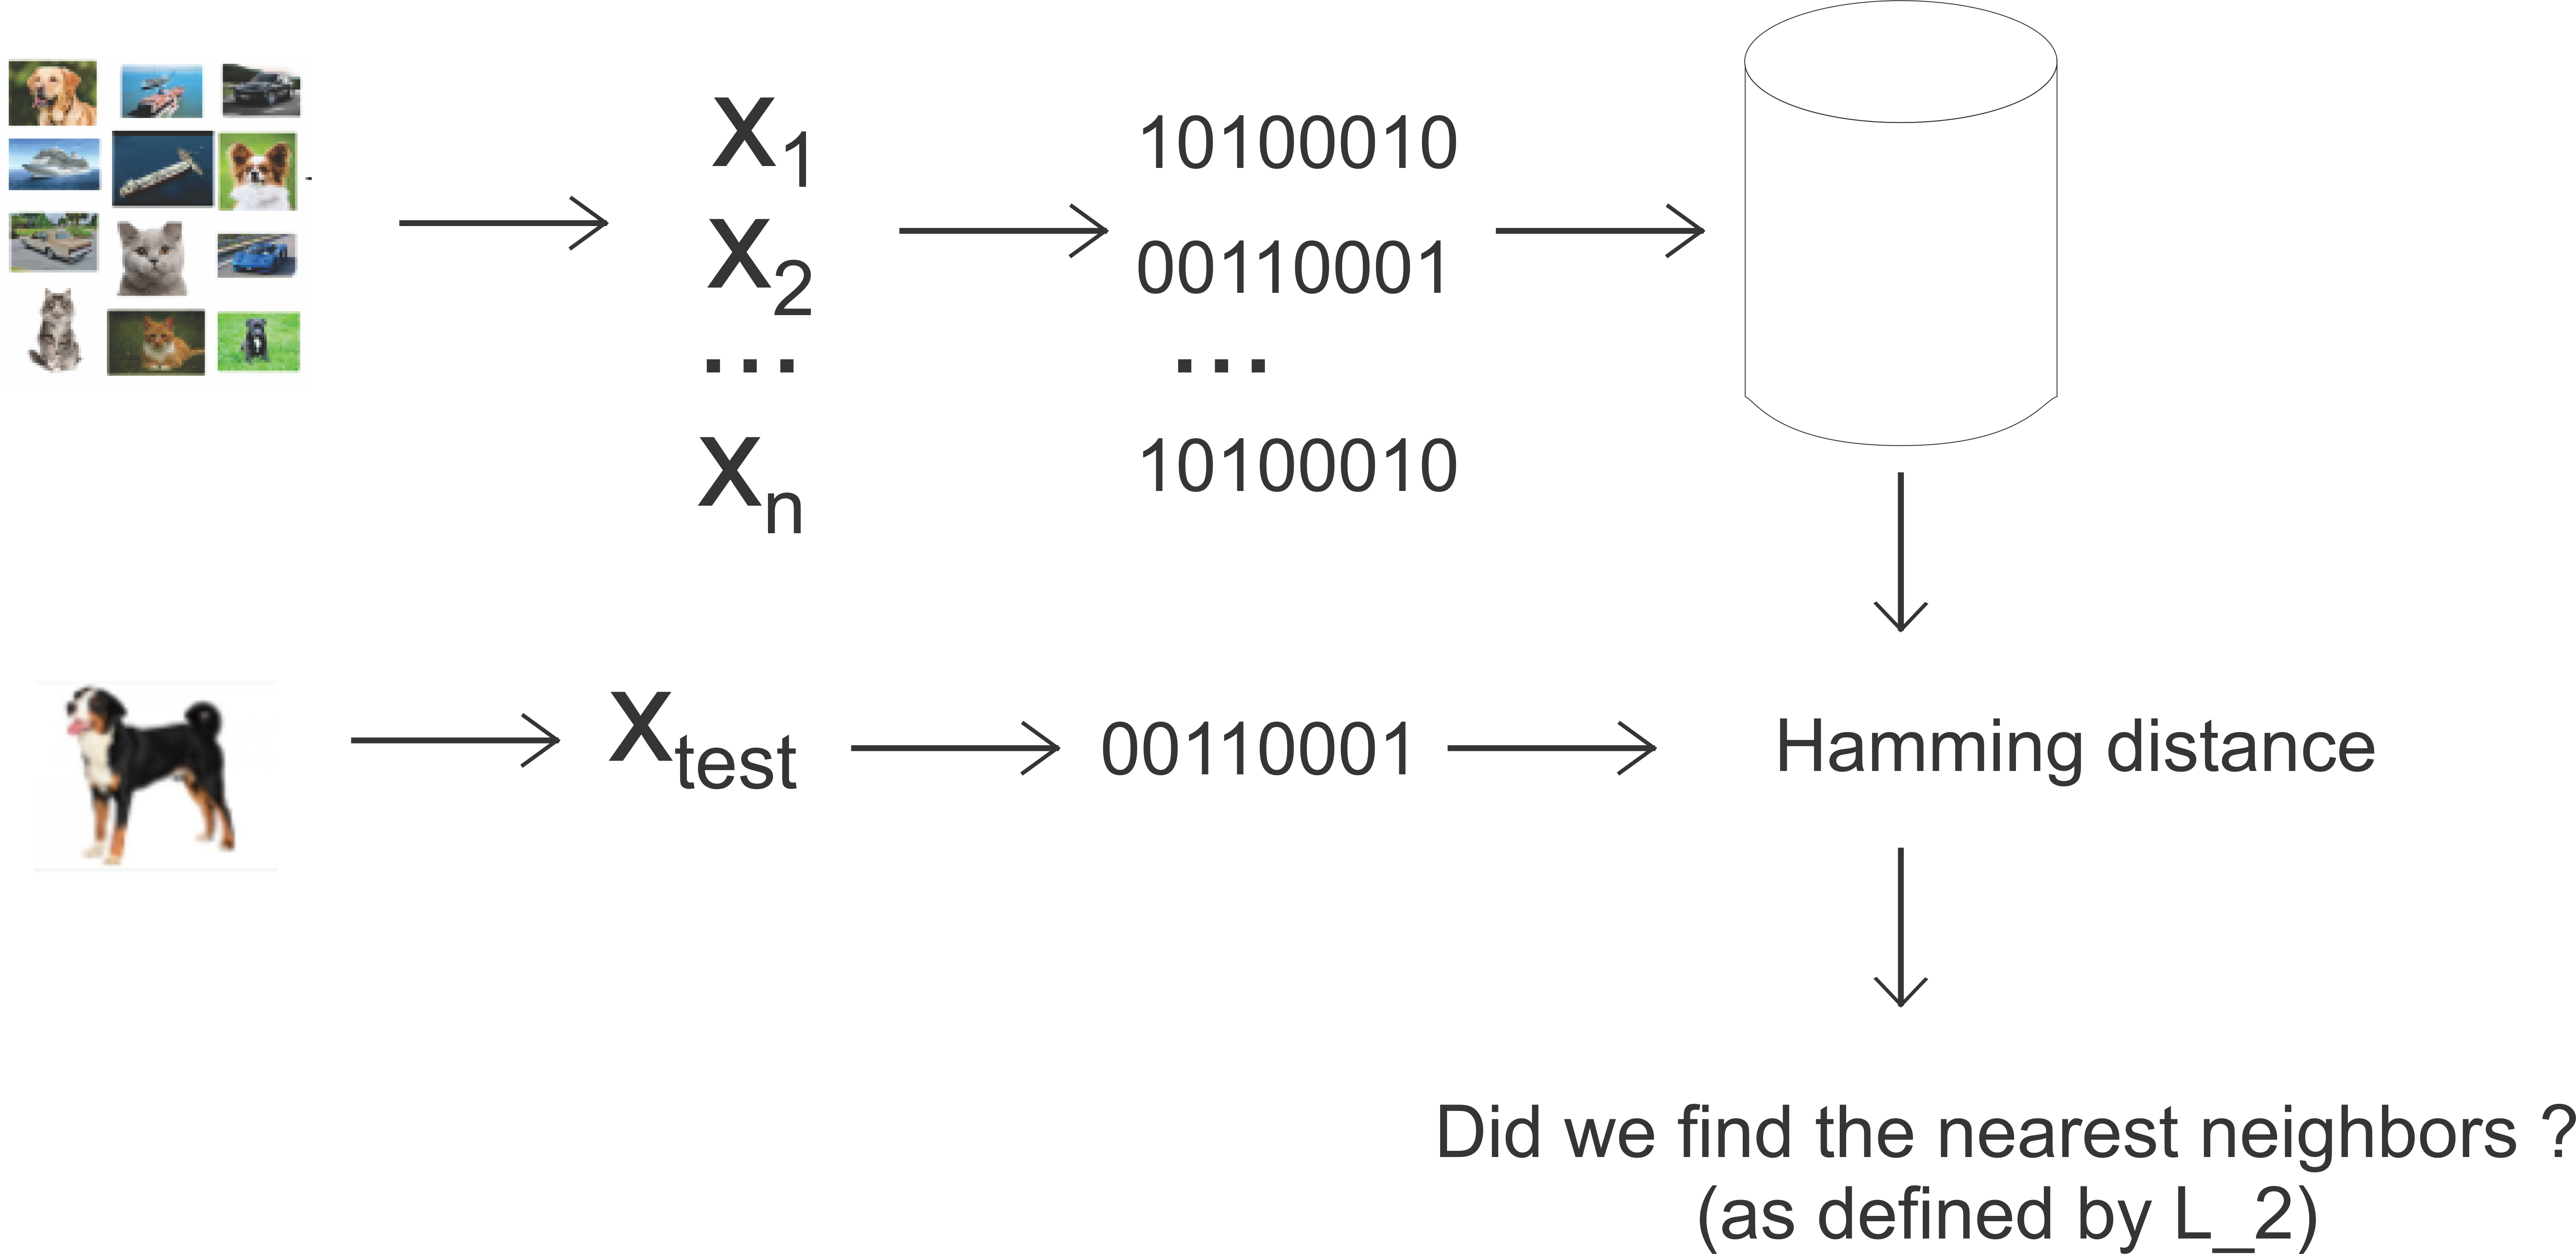
\includegraphics[width=8cm]{dash/11.PNG}
\centering
\end{figure}

\textbf{SUPERVISED HASHING}
Compress a set of vectors and their labels  $((x_i,y_2))^{n}_{i=1}, x_1\in \mathbb{R}^{d}, y_1 \in \{1,...,L\} $
\begin{figure}[htp]
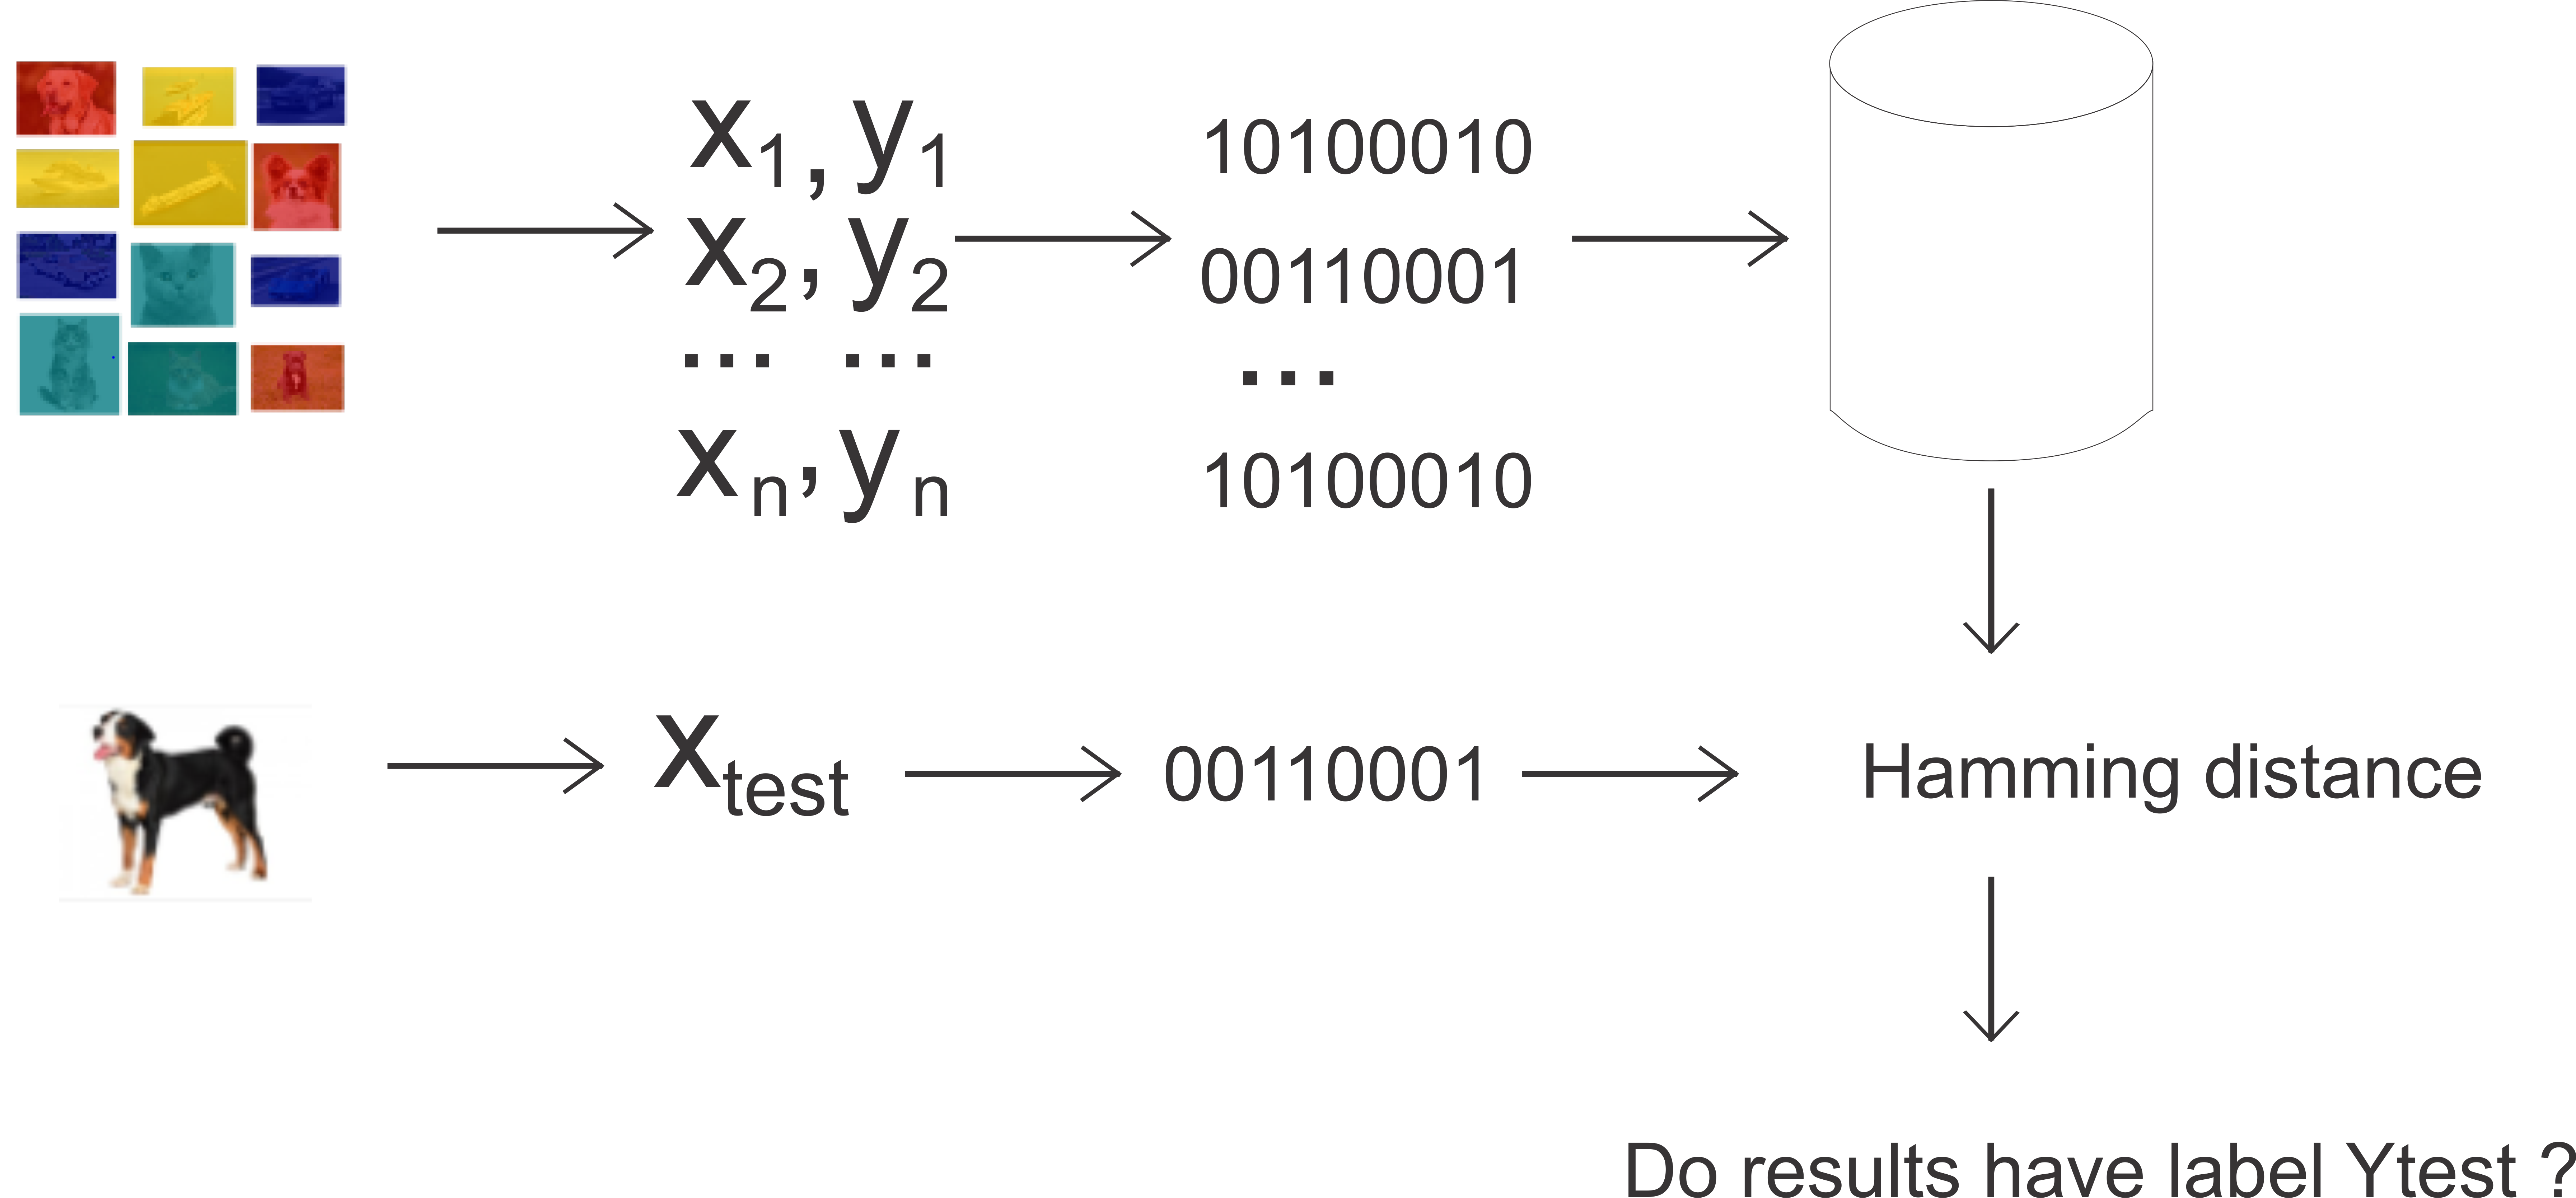
\includegraphics[width=8cm]{dash/12.png}
\centering
\caption{ HASHING FOR NEAREST NEIGHBOR SEARCH }
\end{figure}

\begin{itemize}
\item Supervised hashing $[1, 2]$: labels $y$ known for all $x$ in the reference set
\item Semi-supervised hashing $[3, 4]$: labels $y$ known for only $n_label$ samples
\end{itemize}

 
 This paper proposes a novel supervised hashing technique,  named  Deep frActal based  Hashing (DAsH),  designed to perform scalable approximate similarity search. The contributions of our work are as follows. First,  we introduce and define a  scheme based on CNN and optimized using fractal theory. To overcome the limitation of large activations on lower layers of CNN (output of the last convolutional layer) we reduce its dimensionality using autoencoders  to the optimal sub-space. Then we index this new representation with LSH scheme.  Second, we present a novel method, based on fractal theory, which allow us to can find the optimal number of hash functions for an approximate similarity search scheme based on LSH.

 
The paper is organized as follows. Section 2 summarizes the background for this work. Section 3 describes the proposed technique and Section 4 reports experimental results on real and synthetic datasets. Finally, we conclude in Section 5.
 
 % todos
\section{Preliminaries}

\subsection{Representation}  % jose luis
     	
Existen varios métodos para representar series temporales, las cuales dan soporte a las búsquedas por similitud y tareas de minería de datos. Estos métodos pueden ser representados en dos categorías: representaciones de Data Adaptativa y representaciones de Data No Adaptativa \cite{wang13}.  

En la representación de Data Adaptativa tenemos los siguientes metodos: Decomposición de Valor Singular (SVD)  que transforma la serie temporal $A_i$ en otra serie temporal $B_i$ de longitud $n$ cuyos elementos están en  orden decreciente \cite{Bettaiah14}, Análisis de Componentes Principales (PCA) que mplica procedimientos matemáticos que transforman un número de (posibles) variables correlacionales en un número (menor) de variables no correlacionadas llamadas componentes principales \cite{wekwek}, en PCA la data es resumida como una combinacion lineal de conjuntos de vectores ortonormales, PCA trbaja de forma similar a  Autoencoders (AE) , SAX permite que una serie temporal de longitud arbitraria n se reduzca a una cadena de longitud arbitraria $ w $, ($ w <n $, normalmente $ w \ll n $) \cite{Lin07} e indexacion de aproximación lineal por partes (IPLA)  que indexa los datos reducidos para acelerar la eficiencia de recuperación de la búsqueda de similitud \cite{Chen07}.

Los metodos mas comunes usados en representacion de data no adaptativa son:  Transformación Discreta de Coseno (DCT) es una transformación ortonormal real. DCT es similar a la transformada de Fourier discreta (DFT), con la diferencia de que utiliza funciones coseno en lugar de senos y cosenos para transformar del dominio del tiempo al dominio de la frecuencia \cite{Bettaiah14}, Transformación de Wavelet Discreta (DWT) procesa datos a diferentes escalas o resoluciones en contraste con DFT \cite{Faloutsos94} donde sólo se consideran los componentes de frecuencia.\cite{Bettaiah14} y Piecewise Aggregate Approximation (PAA).



\subsubsection{Principal component analysis(PCA)}
Principal Component Analysis (PCA) involves mathematical procedures that transforms a number of possible correlational variables into a small number of uncorrelated variables called \textit{principal components}. The first component represents as much variability in the data as possible, and each successive component represents as much of the remaining variability as possible. \\

In PCA, the data is summarized as a linear combination of a set of orthonormal vectors. Let $\{ x_i \}_{i=1}^n$  a sample of $ \mathbb{R}^d $  with mean $\bar{x}$  and covariance $ \sum $, with spectral decomposition $ \sum = U \Lambda U^T $.

The main transformation component $y= U^T(x-\bar{x})$  produces a reference system in which the sample has a mean $ 0 $ and a covariance matrix $\Lambda$ containing the eigenvalues of $\sum$. Now, we can discard the variables with small variance to project them on a subspace covered by the first main component, and get a good approximation of the original sample. The key property of PCA is to achieve the best linear mapping $x \in \mathbb{R}^d \rightarrow x^* \in \mathbb{R}^m$ of the sum of least squares errors in the reconstruction of data.

\subsubsection{Factor Analysis}
Factor analysis is a statistical method for modeling the covariance structure of high dimensional data using a small number of latent variables \cite{Ghahramani}. The data are assumed to be a linear combination of uncorrelated Gaussian sources (factors). After the linear combination, each component of the data vector is also assumed to be corrupted with additional Gaussian noise. (see Figure \ref{fig:fig_1} )
\begin{figure}[htp]\centering
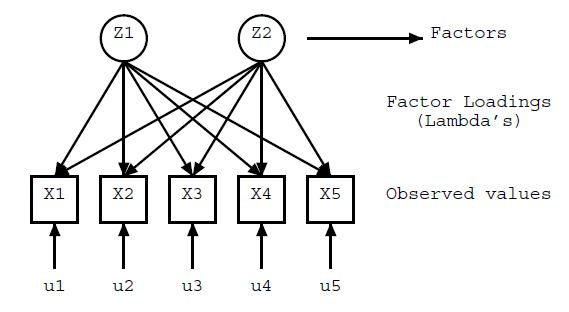
\includegraphics[width=0.6\columnwidth]{images_fractal/frac_1.JPG}
\caption{ Simple route diagram for a factor analysis model }
\label{fig:fig_1}
\end{figure}

The objective of the factor analysis is to find $\Lambda$ and $\Psi$ which improves the model of the $ x $ structure. The factorial variables $ z $ of the correlation model between the elements of $ x $, while the variable $ u $ counts for an independent noise in each element of $ x $. The $ m$ factors play the same role of principal components in the PCA. We first subtract the information from the data and then show the date as:
\begin{equation}
    x - \mu = \Lambda z + u
\end{equation}

\subsubsection{Self Supervised Multi Layer Perceptrons(AUTOENCODER)}
The supervised MLP architecture, or also called autoencoder, implements a mapping using two layers of linear perceptrons with $ d $ input, $ m $ hidden units and $ d $ training outputs to replicate the input to the output layer minimizing the error Of the sum of squares with \textit{backpropagation}. This approach is called \textit{self-supervised}, referring to the fact that during training each vector output sample is identical to the vector input sample.
\begin{figure}[htp]\centering
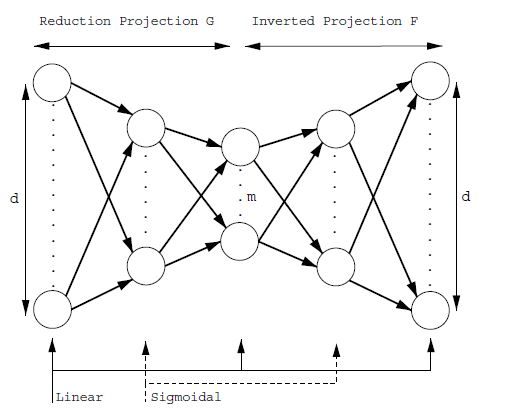
\includegraphics[width=0.6\columnwidth]{images_fractal/frac_2.JPG}
\caption{ The self-supervised MLP architecture }
\label{fig:fig_2}
\end{figure}

A botleneck MLP with a unique hidden layer physically performs a linear PCA even with non-linear hidden units. In fact, in order to effectively implement a non-linear dimensionality reduction, the mapping function $ F $ and $ G $ must be both non-linear. The process of dimensionality reduction consists to find the functions $ F $ and $ G $ which are approximately functions inverse to each other. Since the inverse of a nonlinear function can not be linear, therefore, if any of the functions is linear, the other must also be linear.

Linear self-supervised MLP can be extended to implement a non-linear PCA, using non-linear activation functions and more hidden layers (see Figure \ref{fig:fig_2}).

     	
\subsubsection{Fractal Theory } % jose luis
 

A fractal is characterized by the self-similarity property, i.e., it is an object that presents roughly the same characteristics when analyzed over a broad range of scales \cite{DBLP:journals/jidm/TrainaTWF10}. From the Fractal Theory, the Correlation Fractal Dimension $\mathfrak{D}$ is particularly useful for data analysis, since it can be applied to estimate the intrinsic dimension of real datasets that exhibit fractal behavior, i.e., exactly or statistically self-similar datasets \cite{DBLP:fractal2016}.   It has been shown that, given a set of $N$ objects in a dataset with a distance function $d(x,y)$, the average number of $k$ neighbors within a given distance $r$ is proportional to $r$ raised to $\mathfrak{D}$. Thus, the pair-count $PC(r)$ of pairs of elements within distance $r$ follows the power law:
\begin{equation}\label{eq:fractal}
       PC(r) = K_p \times r^{\mathfrak{D}}
    \end{equation}

     where, $K_p$ is a proportionality constant, and $\mathfrak{D}$ is the correlation fractal dimension of the dataset.
    Consequently, a fractal is defined by the self-similarity property, that is the main characteristic that represents exactly or statistically  the similarity between the parts to the whole fractal.
 
\subsubsection{ Fractal Dimension and Dimensionality Reduction} % jose luis
 

The approaches used to reduce dimensionality depend on some parametric and non-parametric methods. Other methods reduce the original feature space by heuristic deletion of some of the attributes.


\subsection{Retrieval Performance} % supervised hashing %% theoria 

%% Protocol 1: Retrieval of unseen classes

\subsubsection{Evaluation Protocols} % carlos

 
%This section describes the protocols used in the literature for SSH and SH, and discuss how a simple strategy efficiently solves the corresponding problems.

In this section, we describe the protocols used in the literature for SSH and SH and explain how a simple strategy efficiently solves the similar problems.

\subsubsection*{Evaluation protocols of SSH and SH}

%The task of SSH consists in indexing a dataset of $N$ images $\mathcal{I}_{train}$, of which a subset $\mathcal{I}_{label} \subseteq \mathcal{I}_{train}$ is labeled.  SH is the extreme case $\mathcal{I}_{label} = \mathcal{I}_{train}$. Given an unlabeled query image $q$, the system must return an ordered list of images from the $\mathcal{I}_{train}$. For evaluation purposes, a dataset of queries is given; the labels of the queries as well as all labels in $\mathcal{I}_{train}$ are known to the evaluator, even in the SSH setting, and an image is deemed correct if it has the same label as the query. The performance is measured in terms of precision or mean average precision (mAP), which we now describe.
SSH consists in index a dataset of $N$ images $\mathcal{I}_{train}$, of which a subset $\mathcal{I}_{label} \subseteq \mathcal{I}_{train}$ is labeled.  But, SH is the extreme case $\mathcal{I}_{label} = \mathcal{I}_{train}$. If we have an unlabeled query image $q$, the system have to return an ordered list of images from the $\mathcal{I}_{train}$. To evaluate, we have a dataset of queries; the evaluator knows all labels of the queries as well as the labels in $\mathcal{I}_{train}$, also in the SSH setting, then an image is considered correct if it and query have the same label. The performance is measured by precision or mean average precision (mAP).

%Given a query $q$, we first define $\delta (q, i)=1$ if the $i^{th}$ image is correct for $q$, and $0$ otherwise. The precision at (rank) $k$ is given by $P(q,k) = \tfrac{1}{k} {\sum}_{i=1}^{k} \delta (q, i)$. Denoting by $cl(q) = {\sum}_{i=1}^{N} \delta (q, i)$ the total number of correct images in $\mathcal{I}_{train}$, the average precision at $k$ is $AP(q, k) = \tfrac{1}{cl(q)}{\sum}_{i=1}^{k}\delta (q, i) P(q,i)$. The mAP at $k$ (or simply mAP when $k = N$) is the mean AP over all test queries.
Then, given a query $q$, if the $i^{th}$ image is correct for $q$ we define $\delta (q, i)=1$ , and $0$ otherwise. The precision at (rank) $k$ is given by $P(q,k) = \tfrac{1}{k} {\sum}_{i=1}^{k} \delta (q, i)$. Denoting by $cl(q) = {\sum}_{i=1}^{N} \delta (q, i)$ the total number of correct images in $\mathcal{I}_{train}$, and the average precision at $k$ is $AP(q, k) = \tfrac{1}{cl(q)}{\sum}_{i=1}^{k}\delta (q, i) P(q,i)$. The mAP at $k$ (or simply mAP when $k = N$) is the mean AP over all test queries.

\subsubsection*{Retrieval through class probability estimation}

%The information retrieval \cite{doi:10.1108/eb026647} and learning to rank that the optimal prediction for precision at $k$ is given by ranking items $x \in \mathcal{I}_{train}$ n according to their probability of being correct for the query. This result extends to the optimization of $mAP$.

The information recovery \cite{doi:10.1108/eb026647} and learning to rank that the best prediction for precision at $k$ is given by placing items $x \in \mathcal{I}_{train}$  $n$ according to the chance of being correct for the query. This result presents to the optimization of $mAP$.
\\
%\textbf{Optimal ranking for SH.} In the specific setup of SH where the system knows the labels of the images in $\mathcal{I}_{train}$, the probability that an image $x$ with label $y$ is correct is the probability $\mathbb{P}(y\mid q)$ that the query image has label $y$. The important point here is that the probability of $x$ being correct for $q$ only depends on the label of $x$. Thus, ordering the $C$ labels so that $\mathbb{P}(y\mid q)\geq \dots \geq\mathbb{P}(c_C\mid q)$,the optimal ranking is to return all images of $\mathcal{I}_{train}n$ with label $c_1$ first, followed by all images with label $c_2$, and so on.
\textbf{Optimal ranking for SH.} In the particular setup of SH where the system knows the labels of the images in $\mathcal{I}_{train}$, the probability that a picture $x$ with label $y$ is correct is the likelihood $\mathbb{P}(y\mid q)$ that the query image has label $y$. The important point in this part is that the probability of $x$ being correct for $q$ only depends on the label of $x$. Thus, ordering the $C$ labels so that $\mathbb{P}(y\mid q)\geq \dots \geq\mathbb{P}(c_C\mid q)$, the best ranking is to return the complete dataset of $\mathcal{I}_{train}n$ with label $c_1$ first, followed by all the pictures with label $c_2$, and so on.
\\
\begin{comment}
In practice, $\mathbb{P}(.\mid q)$ is unknown, but we can train a classifier
on $\mathcal{I}_{label} = \mathcal{I}_{train}$ which outputs probability estimates $\hat{\mathbb{P}}(c\mid q)$ for every label $c$, and compute the optimal ranking according to $\hat{\mathbb{P}}(c\mid q)$ Such probability estimates are given by,
e.g., multiclass logistic regression or a Convolutional Neural
Network (CNN) with a softmax output layer. Labels of $ \mathcal{I}_{train}$
are stored on [$log2 (C)$] e bits or in an inverted file.
\end{comment}

In practice, $\mathbb{P}(.\mid q)$ is unfamiliar, but we can train a classifier on $\mathcal{I}_{label} = \mathcal{I}_{train}$ which outputs probability con predict $\hat{\mathbb{P}}(c\mid q)$ for every label $c$, and process the optimal ranking according to $\hat{\mathbb{P}}(c\mid q)$ Such probability estimates are shown by, e.g., multiclass logistic regression or a Convolutional Neural Network (CNN) with a softmax output layer. Labels of $ \mathcal{I}_{train}$ are stored on [$log2 (C)$] e bits or in an inverted file

\\
%\textbf{Relationship between classification accuracy and ranking performance.} If we denote the classification accuracy as $p$, then the resulting mAP is at least $p$. When the classifier predicts the class of $q$ correctly, all images of that class will be ranked first and the resulting AP($q$) is $1$; this happens on a proportion $p$ of the queries. So, the classification accuracy is a lower bound on the mAP.

\textbf{Relationship between classification accuracy and ranking performance.} If we show the classification accuracy as $p$, so the resulting $mAP$ is at least $p$. When the classifier foretells the class of $q$ correctly, all images of this data set will be listed first, and the resulting AP($q$) is $1$; this occurs on a proportion $p$ of the queries. So, the classification accuracy is a lower bound on the mAP.
\\
%\textbf{Optimal ranking for SSH.} In the more general setup of SSH, we do not know the label of some images in $\mathcal{I}_{train}$. Yet, considering the (true) conditional label probabilities $\mathbb{P}(c\mid q)$ and $\mathbb{P}(c\mid x)$, the probability that $x$ is correct for $q$ is given by $\sum_{c=1}^C \mathbb{P}(c\mid q) \mathbb{P}(c\mid x) $ it is the probability that both q and x have the same label, assuming conditional independence of the labels of the query and the image. Notice that this is the dot product between the conditional label probability vectors of $q$ and $x$.Then, given probability estimates $\hat{\mathbb{P}}$  for the labels of queries and images, which are obtained on $\mathcal{I}_{label}$, we consider two retrieval algorithms:

\textbf{Optimal ranking for SSH.} In the more general setup of SSH, we do not know the label of some images in $\mathcal{I}_{train}$. Yet, considering the (real) probabilities $\mathbb{P}(c\mid q)$ and $\mathbb{P}(c\mid x)$, the probability that $x$ is correct for $q$ is given by $\sum_{c=1}^C \mathbb{P}(c\mid q) \mathbb{P}(c\mid x) $ it is the probability that both q and $x$ have the same label, assuming conditional self-sufficiency of the labels of the query and the image. Notice that this is the dot product between the dependent label probability vectors of $q$ and $x$. Then, given probability measures $\hat{\mathbb{P}}$  for the labels of queries and images, which are taken on $\mathcal{I}_{label}$, we consider two retrieval algorithms:

\\
\begin{itemize}
%\item \textbf{Classifier topline: }: For each image $x$of $\mathcal{I}_{train}$, store a vector $u(x)$ equal to either (1) the one-hot encoding vector of the label of $x$ if $x \in \mathcal{I}_{label}$, or (2) the full conditional probability vector  $\hat{\mathbb{P}}(.\mid x)$). Rank images $x$ according to the dot product $\langle\hat{\mathbb{P}}(.\mid q), u(x)\rangle$  This strategy corresponds to the optimal strategy, but requires storing the probability vectors for images in $\mathcal{I}_{train} \backslash \mathcal{I}_{label}$

\item \textbf{Classifier topline: }: For each image $x$of $\mathcal{I}_{train}$, saves a vector $u(x)$ either way \cite{norouzi2012hamming} the one-hot encoding vector of the label of $x$ if $x \in \mathcal{I}_{label}$, or \cite{wang2013learning} the full vector  $\hat{\mathbb{P}}(.\mid x)$). Rank images $x$ according to the dot product $\langle\hat{\mathbb{P}}(.\mid q), u(x)\rangle$  This strategy corresponds to the best strategy, but needs to save the probability vectors for each image in $\mathcal{I}_{train} \backslash \mathcal{I}_{label}$

%\item \textbf{Classifier hashed: } Here we hash the conditional probability vector. The first hashing method that we evaluate, is the one-hot strategy, which stores the index of the maximal activation on $\left \lceil log_2(C) \right \rceil$ bits. This approach, denoted \textbf{Classifier+one-hot} in what follows, returns all images of the strongest class first. The second encoding, referred to as Classifier+LSH, is locality-sensitive hashing (LSH) with tight frames \cite{jegou2012anti}, a simple non data adaptive hashing scheme. This LSH method produces binary vectors that are compared with Hamming distances. Therefore it can be used as drop-in replacements for the competing binary encoding methods.

\item \textbf{Classifier hashed: } Here we hash the probability vector. The first hashing method that we evaluate is the one-hot strategy, which saves the index of the maximal activation on $\left \lceil log_2(C) \right \rceil$ bits. This approach expressed \textbf{Classifier+one-hot} in what results, returns all images of the strongest class first. The second encoding, referred to as Classifier+LSH, is locality-sensitive hashing (LSH) with tight frames \cite{jegou2012anti}, a simple non-data adaptive hashing scheme. This LSH method provides binary vectors that are compared with Hamming distances. Consequently, it can be used as drop-in replacements for the competing binary encoding methods.
\end{itemize}















   
\section{Comparison of Data Representations} % Ricardo
   
      (MNIST, CIFAR 10, SVHN, AG-NEWS) ///
   \subsection{Fractal Dimension and Dimensionality Reduction (en proceso)}
      	All methods referenced in section 2.1. (MNIST, CIFAR 10, SVHN, AG-NEWS)
   \subsection{Analysis of Classification Accuracy}
%      	Classification Accuracy
%     	  	 [Original_dim,    optimal_dim  - 1, optimal_dim,  optimal_dim + 1]
%            	  mnist_800.train.csv   mnist_50. train.csv  mnist_64. train.csv %mnist_90. train.csv
%            	  mnist_800.test.csv   mnist_50. test.csv  mnist_64. test.csv %mnist_90. test.csv
%[**** muestra / poblacion *****]
%     	(MNIST, CIFAR 10, SVHN, AG-NEWS)  vs (MNIST, CIFAR 10, SVHN, %AG-NEWS)_optimal_dim
 


\subsection{Accuracy of Similarity} % Oscar

In this section, we are going to do a review of the methodolody of our evaluation, as well as the parameters that we use for each similarity measuares, then presents the results and the discuss of what we find.

\subsubsection{Accuracy Evaluation Framework}

      
The idea is to work with a nearest neighbor (1NN) classifier [17, 32] on labeled data to evaluate the efficacy of the distance measure. Specifically, each time series has a correct class label, and the classifier tries to predict the label of its nearest neighbor in the training set.  

To evaluate each similarity measure, we have to use a cross-validation algorithm ( ), based on [37]. Using a layered divided randomly the input data set into $k$ subsets for the organization based on subsequences to reduce the impact of skewed class distribution. 

This algorithm requires that we provide an input k for the number of cross-validations.  Each data set tries to strike a balance between the following factors:  1. The training set size should be selected to enable discriminatively, i.e., 2. a number of items in the training set should be sufficient to represent each class, and 3. The number of cross-validations should be between 5− 20 to minimize bias and variation[28]. 

The actual number of splits is empirically selected such that the training error for 1NN Euclidean distance (which we use as a comparison reference) However, most of the time only empirical values are given for each parameter in isolation. 

In our experiments we consider both the version of distance measures without warping and with warping.  We fix the matching reward weight to 50 and search for the optimal penalty weight from 0 to 50, as suggested by the authors.







\subsubsection{Analysis of Classification Accuracy}
To provide a general evaluation, we described the performs presented in \cite{ding2008querying}, they experiment on time series data sets. First, they compared the different variances of $L_p$ -norms, they found that the Euclidean distance and the Manhattan distance have a very close performance, and both largely outperforms the $L_{\infty}$ -norm. Due to the $L_{\infty}$ -norm uses the maximum distance between two sets of time series points, it is more sensitive to noise.

In \cite{ding2008querying} the authors have found that full DTW is superior over Euclidean. And the effectiveness of constrained DTW is the same than that of full DTW. So, to decrease the time to get the distance and to use proposed lower bounding techniques, it could generally use the constrained DTW instead of DTW. 

On the other hand, the accuracy of DISSIM is slightly better than Euclidean distance. On most of the data sets, TQuEST is worse than Euclidean and DTW distances. The performance of LCSS, EDR and ERP outperform Euclidean distance by a large percentage. Only EDR is potentially slightly better than full DTW, while the performance of LCSS and ERP are very close to DTW. It has observed that the constrained version of LCSS is even slightly better the unconstrained one, while it also reduces the computation cost and gives increase to an efficient lower-bounding measure.

The authors in \cite{ding2008querying} observed that the accuracy of SpADe is close to that of Euclidean but is inferior to DTW distance, although on some data sets SpADe outperforms the other two. In summary, they found through experiments that there is no clear evidence that there exists one similarity measure that is superior to others in the literature, regarding accuracy. 



\section{Comparison of Retrieval Performance} % Jose Luis
   
\subsection{Evaluation Protocol: Retrieval with hash codes}
LSH, Lsh-forest, ITQ, LOPQ. (MNIST, CIFAR 10, SVHN, AG-NEWS)     
            	Accuracy  [Recall]( Result [exact-kNNQ vs ann-kNNQ]), Precision & Recall, mAP [].
 

  
%\subsection{Evaluation Protocol: Retrieval with hash codes}
 

In this section, we describe the two evaluation tasks proposed in \cite{sablayrolles2016should}, namely retrieval of unseen classes, and transfer learning to new classes. They correspond to application cases on large datasets. The two protocols differ only in the evaluation metric: ranking versus class accuracy.

\textbf{Dataset definition.} at test time we use separate classes from a standard classification dataset. When learning the hashing function $75\%$ of the classes are assumed to be known, and the $25\%$ remaining classes are used to evaluate the encoding/hashing scheme. We call train75/test75 the train/test images of the $75\%$ classes and train25/test25 the remaining ones.

\textbf{Protocol 1: Retrieval of unseen classes}, to index train25 and use test25 as queries, we use the hashing scheme. We use the labels of train25 for evaluation only. This setup is like an instance search approach except that the class labels give the ground-truth. The train75 - train25 - test25 split is the supervised equivalent of the learn - database - query split in unsupervised hashing.

\textbf{Protocol 2: Transfer learning, } the authors proposed to train a new CNN from scratch with the same structure as the top of the original network, using the stored train25 descriptors. The goal is to maximize the transfer accuracy on test25.
   
  % LSH, Lsh-forest, ITQ, LOPQ. (MNIST, CIFAR 10, SVHN, AG-NEWS)     
   %         	Accuracy  [Recall]( Result [exact-kNNQ vs ann-kNNQ]), Precision & Recall, mAP [].
            	
 
 \begin{table*}[ht]
\caption{Experimentos con data normalizada MNIST, SVHN . }
\label{table:map}
\centering
\begin{footnotesize}
\begin{tabular}{l|c|c|c|c|c|c|c|c|}
\cline{2-9}
                                           & \multicolumn{4}{c|}{\textbf{MNIST}}             & \multicolumn{4}{c|}{\textbf{SVHN}}         \\ \cline{2-9} 
                                           & \textbf{mAP} & \textbf{Precision} & \textbf{Recall} & \textbf{Accuracy} & \textbf{mAP} & \textbf{Precision} & \textbf{Recall} & \textbf{Accuracy}  \\ \hline
\multicolumn{1}{|l|}{\textbf{BF Blass  \cite{multiprobe}}}       & 0.32         & 0.10            & 0.99    & 1.0      & 0.33         & 0.11            & 0.99  & 1.0     \\ \hline
\multicolumn{1}{|l|}{\textbf{MpLSH \cite{itq}}}         &  0.006         & 0.0007            & 0.006    & 0.0007   & 0.071        & 0.0098            & 0.093   & 0.027    \\ \hline
\multicolumn{1}{|l|}{\textbf{ITQ \cite{lopq}}}        & 0.27         & 0.081            & 0.81    & 0.74    & 0.31         & 0.106            & 0.92   & 0.915      \\ \hline
\multicolumn{1}{|l|}{\textbf{LSH-F \cite{lshforest}}}       &  0.33         & 0.10            & 0.99 & 0.99       & 0.34         & 0.11            & 0.99    & 0.99    \\ \hline
\end{tabular}
\end{footnotesize}
\end{table*}


            	
\begin{table*}[ht]
\caption{Experimentos con data normalizada CIFAR-10 y AGNEWS. }
\label{table:map}
\centering
\begin{footnotesize}
\begin{tabular}{l|c|c|c|c|c|c|c|c|}
\cline{2-9}
                                           & \multicolumn{4}{c|}{\textbf{CIFAR-10}}            & \multicolumn{4}{c|}{\textbf{AGNEWS}} \\ \cline{2-9} 
                                           & \textbf{mAP} & \textbf{Precision} & \textbf{Recall} & \textbf{Accuracy} & \textbf{mAP} & \textbf{Precision} & \textbf{Recall} & \textbf{Accuracy}\\ \hline
\multicolumn{1}{|l|}{\textbf{BF Blass  \cite{multiprobe}}}       & 0.23        & 0.099  & 0.099 & 1.0    & 0.0         & 0.0            & 0.0    & 0.0\\ \hline
\multicolumn{1}{|l|}{\textbf{MpLSH \cite{itq}}}         & 0.003         & 0.0003    & 0.003        & 0.0004      & 0.0         & 0.0            & 0.0    & 0.0  \\ \hline
\multicolumn{1}{|l|}{\textbf{ITQ \cite{lopq}}}        & 0.22         & 0.098            & 0.98  & 0.98      & 0.0         & 0.0            & 0.0    & 0.0\\ \hline
\multicolumn{1}{|l|}{\textbf{LSH-F \cite{lshforest}}}       & 0.23         & 0.099            & 0.99  &  0.99    & 0.0         & 0.0            & 0.0 & 0.0  \\ \hline
\end{tabular}
\end{footnotesize}
\end{table*}



\section{Conclusion \& Future Work}
 

\bibliographystyle{plain}
\bibliography{references}

\end{document}

